
\documentclass[12pt,journal,compsoc]{IEEEtran}
\usepackage{array}
\usepackage{bytefield}
\usepackage{graphicx}
\usepackage{listings}
\usepackage{slashbox}
\usepackage{tikz}
\lstset{
frame=tb,
language=C,
aboveskip=3mm,
belowskip=3mm,
showstringspaces=false,
columns=flexible,
basicstyle={\small\ttfamily},
numbers=none,
breaklines=true,
breakatwhitespace=true,
tabsize=3
}
\hyphenation{op-tical net-works semi-conduc-tor}
\newcounter{mcount}
\setcounter{mcount}{0}
\begin{document}
\title{Chat System\\EN 600.437 Final Project}
\author{David Gong, Stephen Hamilton}% <-this % stops a space
\date{Sunday, September 21, 2014}
\IEEEtitleabstractindextext{%
\begin{abstract}
A distributed chat server system that is fault tolerant through the use of a lamport timestamp.
\end{abstract}
}
\maketitle
\section{Overall Approach}
\IEEEPARstart{T}{his} chat service will be composed of 5 servers each hosting their own set of clients. Servers will communicate with each other and their clients through spread utilizing multicasting with agreed ordering. A client will pick some server to which to connect depending on server availaiblity. Then the client selects a username which is a unique identifier (meaning other client process running with the same name will be treated as one person). Finally a client joins the the desired chat room to chat with other clients that joined that chatroom.

All operation ordering is done on the server side. The client simply makes requests for its desired information and the server sends it what it needs. Therefore, the client will not see that its request has been fulfilled until the server has completely processed it. There is no computation done on the client side. Rather, the only thing the client must do is maintain the linked list of messages which exist in the chat room of which it is a member.

Now in order to maintaining global consistency across servers, we incorporate a lamport timestamp into the requests made by a client. By using a lamport timestamp which consists of a process ID and a process sequence number, we can maintain total ordering across all servers that are connected. Furthermore, the lamport timestamp makes it possible to retain consistent and agreed ordering across partitions and merges.

We also use a matrix to maintain knowledge of the most recent messages each server has from every server. Therefore, from the perspective of some given server, it knows what messages other servers are missing from not only itself but also from all other servers.

By using a lamport timestamp along with this matrix of the highest lamport timestamps received, we can acheive an eventually consistent state across all of the servers.

Next, in order to acheive resiliency in the face of crashes, we simply incorporate a file writing system such that after every update received by some server, whether that is from another server or a client, is written to a file (disk). Therefore, when the crashed process is rejuvinated, it can open the written file and catch itself back up to its state prior to the crash..

\section{Design}
\subsection{Assumptions}
Below are our assumptions.
\begin{itemize}
\item A user is uniquely identified by their username.
\item 
\end{itemize}
\subsection{Group Architecture}
Four kinds of groups are created in order to properly manage this chat service:
\begin{itemize}
\item One server group for all of the servers.
\item One group for each individual server.
\item One group for each individual server and the clients connected to that server.
\item Five groups per existing chat room, one for each server.
\end{itemize}

The group for all of the servers is a group that each server joins. The main use is for communication between the servers. By being a part of the group, servers can receive updates from other servers' clients through those servers. Furthermore, when a partition occurs (some set of servers lose communication with the other set of servers), then the servers know which servers it can still communicate with because those servers that remained in the same partition will see that they are members of the same group.

The groups per server are used for communication from client to server. The server alone joins the group and a client will be able to send requests through this group to the server to which the client is connected.

The groups per server and a server's clients are used for determining whether the server is available or not. A client joins this group when it wants to connect to the corresponding server. If the server is also in that group, then the client knows that the server is availablei. If a server were to disconnect, then clients would be notified that the server they were connected to became unavailable through a membership change notification through the group.

The five groups per existing chat room, one per each server, represents the membership in a given chat room on a specific server. Therefore, when a client decides to join some chat room, it joins this chat room group associated to the client's server. From this, it becomes evident that it becomes the servers' job to maintain consistent communication within chat rooms across servers. The servers are also a part of these chat rooms so that they can determine which clients are in what groups..


\subsection{Message Packet}
% Yair doesn't want code in the design so I guess we just put a discription of the message packet.

We only have one type of packet we send called a chat\_packet. There is a field, "type",on the packet that helps distinguish the role which a given chat\_packet fufills. The different types of packets are as follows:

\begin{enumerate}
\setcounter{enumi}{0}
\item Text chat.
\item Like message.
\item Connection to a server.
\item Receive message.
\item Tell client to display all messages after a given lamport timestamp
\item Request to join a group.
\item Tells the client to refresh the screen with updated messages.
\item Unlike message.
\item Display servers online.
\item Send client user list.
\item Send username/private name combination from server to server.
\item Reove username/private name combination from server to server.
\end{enumerate}

Types 0, 1, and 7 are used both for communcation from server to server and between client and server.

These constitute the main actions that a client can perform in a chat room. A client can say something in a chat room and a client can like/unlike a message in a chat room.

Types 2 and 5 are used for communcation between client and server.

These constitute the packets necessary for setting up a client on a server/chat room. A client thus has a way to tell a server that it wants to connect or that it wants to join a chat room on that server.

Types 4, 6, 8, 9 are used for communcation from server to client.

These constitute the updates that a server must provide a client in order to provide a consistent chat room experience. The server can send updates to the client process that do various things, but in general just keep the client updated on specifically messages and likes from other clients and user changes in a group.

Types 10 and 11 are used for communcation from server to server.

These are specifically for maintaining a consistent view of chat room membership across servers. The servers have types used specifically for communicating changes in users in all of the chat rooms.

%\begin{lstlisting}
%// Structure of chat packet.
%int type;//Type of packet 0 for message, 1 for like
%int sequence; //Sequence of message given to the server
%int server_id; //Server id that the message was created on.
%char name[25]; //Text name of user
%char group[25]; //Text name of chat room
%char text[80]; //Text of chat message
%int like_sequence; //Integer of sequence number of message liked\
%int resend; //Set to 1 if the message is a resend for other servers
%\end{lstlisting}
%The message packet is utilized for both chat messages and likes created by a user.  The message packet will be saved to disk when received from spread, and the sequence number will be assigned upon receiving it from spread (it is null initially).
\newpage

\subsubsection{Server State Machine}
\begin{center}
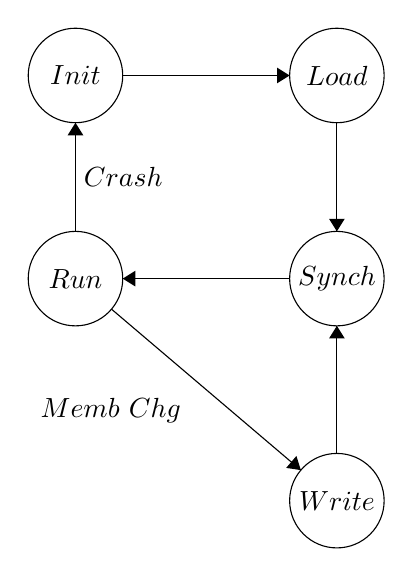
\begin{tikzpicture}[scale=0.2]
\tikzstyle{every node}+=[inner sep=0pt]
\draw [black] (3.3,-3.5) circle (3);
\draw (3.3,-3.5) node {$Init$};
\draw [black] (19.9,-3.5) circle (3);
\draw (19.9,-3.5) node {$Load$};
\draw [black] (19.9,-16.4) circle (3);
\draw (19.9,-16.4) node {$Synch$};
\draw [black] (3.3,-16.4) circle (3);
\draw (3.3,-16.4) node {$Run$};
\draw [black] (19.9,-30.5) circle (3);
\draw (19.9,-30.5) node {$Write$};
\draw [black] (6.3,-3.5) -- (16.9,-3.5);
\fill [black] (16.9,-3.5) -- (16.1,-3) -- (16.1,-4);
\draw [black] (19.9,-6.5) -- (19.9,-13.4);
\fill [black] (19.9,-13.4) -- (20.4,-12.6) -- (19.4,-12.6);
\draw [black] (3.3,-13.4) -- (3.3,-6.5);
\fill [black] (3.3,-6.5) -- (2.8,-7.3) -- (3.8,-7.3);
\draw (3.8,-9.95) node [right] {$Crash$};
\draw [black] (16.9,-16.4) -- (6.3,-16.4);
\fill [black] (6.3,-16.4) -- (7.1,-16.9) -- (7.1,-15.9);
\draw [black] (5.59,-18.34) -- (17.61,-28.56);
\fill [black] (17.61,-28.56) -- (17.33,-27.66) -- (16.68,-28.42);
\draw (5.54,-23.94) node [below] {$Memb\mbox{ }Chg$};
\draw [black] (19.9,-27.5) -- (19.9,-19.4);
\fill [black] (19.9,-19.4) -- (19.4,-20.2) -- (20.4,-20.2);
\end{tikzpicture}
\end{center}

\subsection{Server Data Structures}
The server has two primary data structures. An array of linked lists for all user updates and a linked list of all chat rooms.

\subsubsection{Array of Linked List}
This is an array of length 5, each cell corresponding to a linked list of one server's updates. The updates received from a given server are linked together in no particular order along the designated cell of the array. This data structure is used alongside a matrix which carries the highest lamport timestamp received by each server for each server. This makes it so that when there is a merge or partition, the servers know what updates other servers do not have but need.

The array of linked lists is also useful for achieving fault tolerence. A server can write all of the data in this data structure onto disk and simply come back online by first reading all of the updates and then properly updating its matrix. With this, a server can come back to the exact state with which it crashed.


\subsubsection{Linked List of Chat Rooms}
A second data structure is used in order to keep track of messages (in order) in every chat room. At the highest level, this is a linked list of chat rooms in no particular order. These chat rooms each contain the name string of the chat room it represents and two linked.

There are two linked lists which have different purposes. First, there is a linked list of names used to keep track of the clients (and their usernames) who are a part of that chat room. Each of these names has a name string, a pointer to the next name, and a pointer to a linked list of private names which are unique to each client process. This linked list of private names is used to keep track of the client processes that share the same username (this goes along with the assumption that usernames are unique). This way, when there are no private usernames left in the list, then it is definite that there are no users in that chat room with the associated username.

The other linked list at the second level is the actual messages sent on that chat room. This linked list is sorted by increasing order based on lamport timestamp. These message nodes therefore have a chat\_packet, a pointer to the next message, and a pointer to a list of likes. The mentioned linked lists from each message contain the name of a user who has liked (or then subsequently unliked) the message, a "like" field which determines whether or not that given user is still liking the message, and a field for the lamport timestamp of the highest like/unlike message from the given user.

The incentive behind having this data structure is that a client process will only ever be in one chat room at a time, therefore it will only want updates that pertain to that chat room. With this three tiered linked list, a server can send a client process the updates for a chat room for a single room without difficulty by iterating through the correct chat room's linked list of messages. And then when sending updated messages to the clients, the server can count the number of actual likes by traversing a given message's linked list of likes and send that as part of the message. Therefore the client does no computational work, it simply figures out where the received packet goes in its data structure which is discussed later.

%\subsection{Server Operations}
%We plan to have each server save every message it receives from a client to disk.  We will also have a file that contains messages from all servers that will be written every time there is a membership change.  Sequence numbers will be assigned to each message when it is received from Spread, and a client will not see their message until the server that put it into spread received the message and has a sequence number assigned to it.  Servers will continue to run during a partition.  When a partition merges, the partition that contained the lowest numbered server will have priority to send.  Each server will send its vector containing the highest number sequence from each server.  Each server will resend the messages from the lowest heard sequence for their server. The ordering will be maintained by the sequence number, and further ordering will be by process id to make all servers consistent. When these messages are sent, the resend flag is set so that these message do not get re-ordered, and then they are just added to the linked list for each server.\\
\newpage
\subsection{Client State Machine}

\subsection{Client Data Structures}
The client only has one data structure. A linked list of the messages that have occured in the chat room to which a client is a member. This makes it very easy for the client process to output the contents of its chat room. Simply iterate through the linked list to print out the messages.


\subsection{Algorithm}

\subsubsection{Regular Case}

The client sends all of its actions through the server in order to communicate with the members in a chat room. The server then communicates these actions to the other servers with which it has contact. Lastly, the server 
\subsubsection{Reconciliation Case}

\end{document}
